\section*{Clustering}

Con los resultados de SOM es razonable aplicar más algoritmos para asignar clases a cada uno de los animales para conseguir una mejor delimitación en cada reducción de orden. En la figura \ref{fig:clustering} se visualizan los resultados de aplicar clustering jerarquico de los tipos tipos single, complete y ward con las reducciones de dimension isomap, LLE y T-SNE.

\begin{figure}[H]
    \centering
    \begin{subfigure}{17cm}
        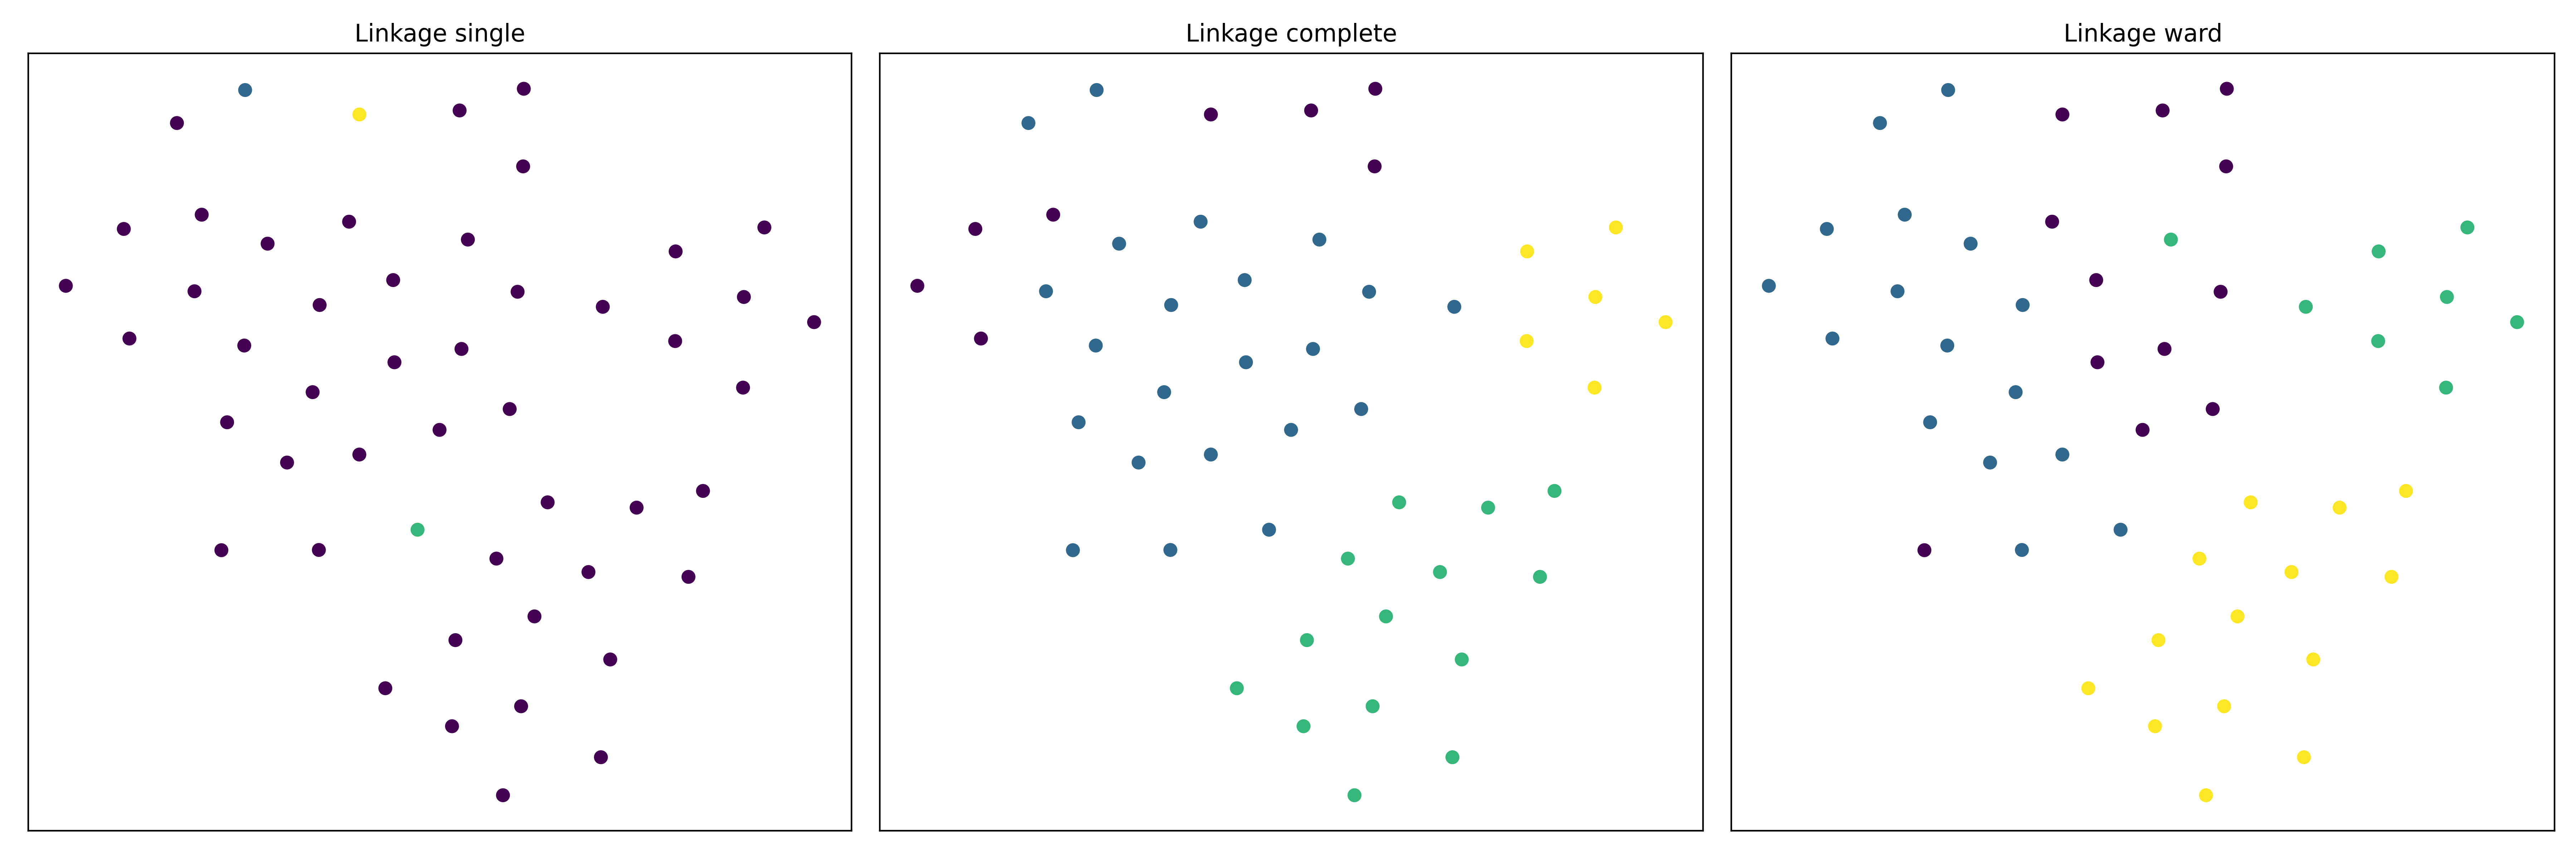
\includegraphics[width=17cm,height=5cm]{Graphics/Cluster_isomap.png}
        \caption{Isomap.}
    \end{subfigure}
    \begin{subfigure}{17cm}
        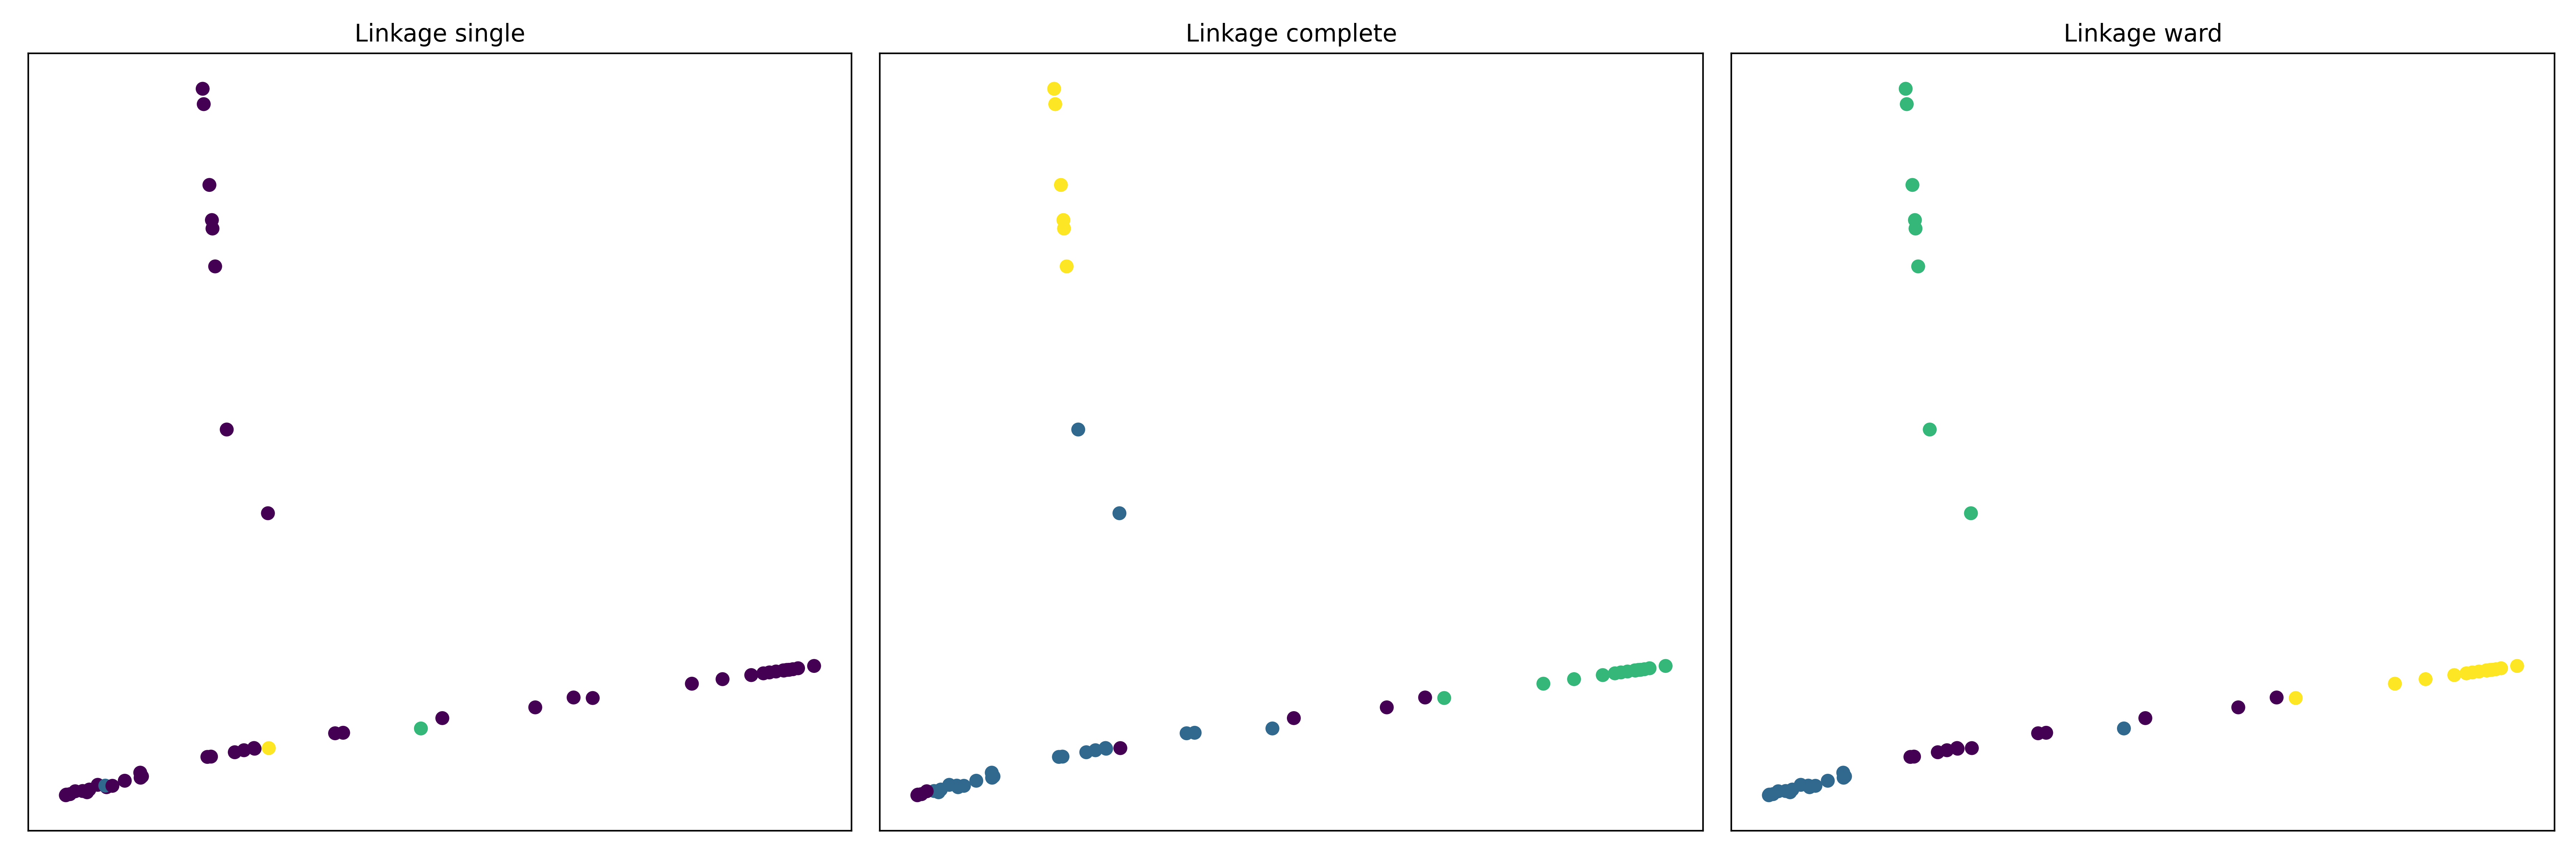
\includegraphics[width=17cm,height=5cm]{Graphics/Cluster_LLE.png}
        \caption{LLE.}
    \end{subfigure}
    \begin{subfigure}{17cm}
        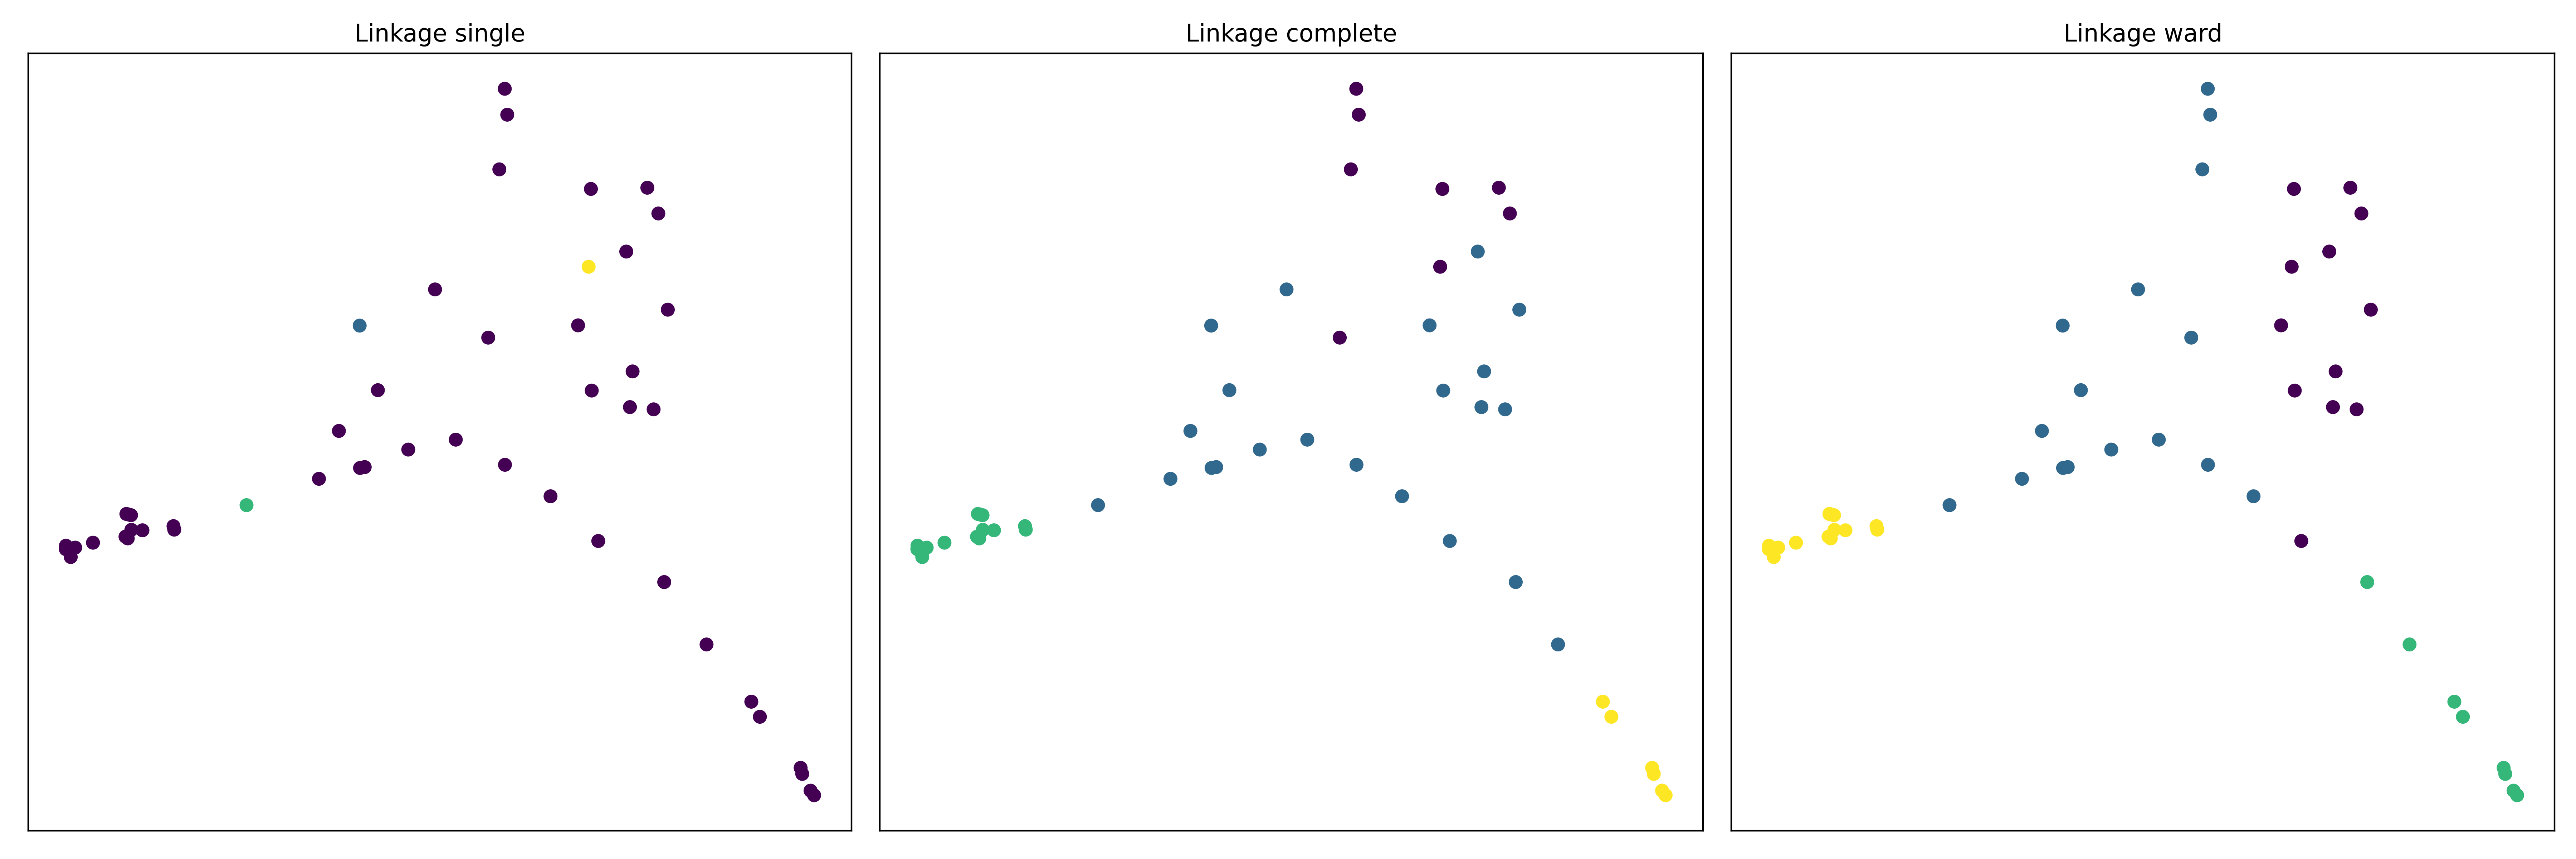
\includegraphics[width=17cm,height=5cm]{Graphics/Cluster_TSNE.png}
        \caption{T-SNE.}
    \end{subfigure}
    \caption{Clustering jerarquico aplicado en conjunto a la reducción de dimension.}
    \label{fig:clustering}
\end{figure}

Con esto se visualiza que los tipos complete y ward obtienen resultados semejantes y con buenas representaciones al hacer una comparación de estos valores con las imagenes de cada animal como se muestran en las figuras \ref{fig:isomap}, \ref{fig:LLE} y \ref{fig:tsne}.


En la figura \ref{fig:denograms} se visualizan los denogramas de cada clustering jerarquico aplicado a cada tipo.

\begin{figure}[H]
    \centering
    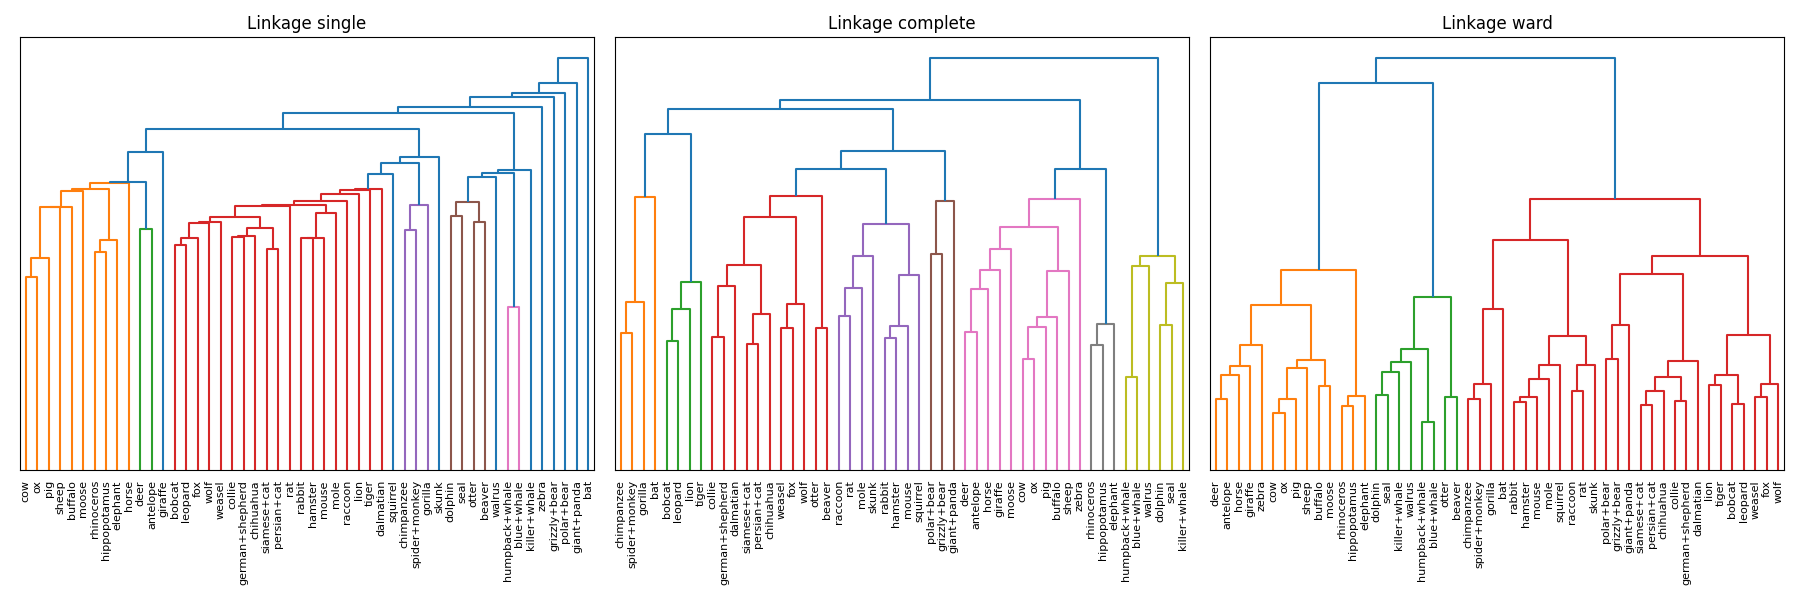
\includegraphics[width=17cm]{Graphics/denograms.png}
    \caption{Denogramas de los clustering jerarquico de tipo single, complete y ward.}
    \label{fig:denograms}
\end{figure}


Con estos resultados se obtiene que los modelos de clustering jerarquico del tipo complete y ward realizan un buen trabajo realizando la asignación de categorias a cada elemento que tenemos. Donde el tipo ward tiene una representación en denograma más sencilla de visualizar e interpretar. Estos modelos llegan a realizar una categorización pero la interpretación que tiene se la damos nosotros, por lo que no se puede especificar sobre que categoria o atributos se pueda hacer un énfasis.